% Created by tikzDevice version 0.12.6 on 2026-08-03 03:40:37
% !TEX encoding = UTF-8 Unicode
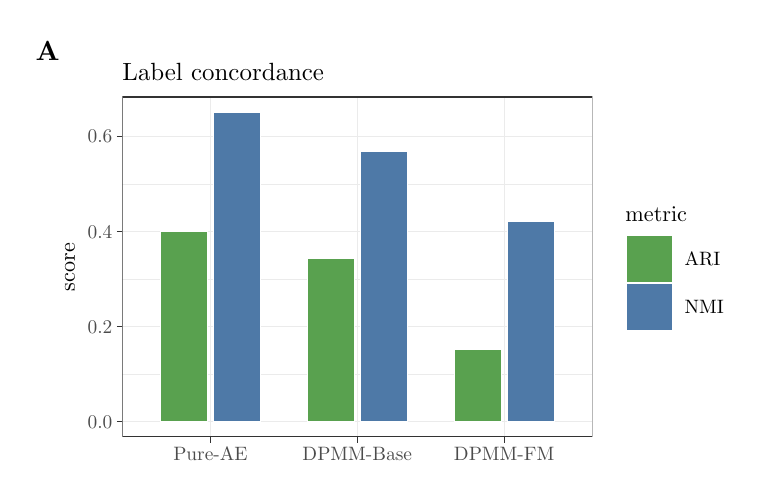
\begin{tikzpicture}[x=1pt,y=1pt]
\definecolor{fillColor}{RGB}{255,255,255}
\path[use as bounding box,fill=fillColor,fill opacity=0.00] (0,0) rectangle (257.09,161.83);
\begin{scope}
\path[clip] (  0.85,  1.74) rectangle (256.24,160.09);
\definecolor{drawColor}{RGB}{255,255,255}
\definecolor{fillColor}{RGB}{255,255,255}

\path[draw=drawColor,line width= 0.4pt,line join=round,line cap=round,fill=fillColor] (  0.85,  1.74) rectangle (256.24,160.09);
\end{scope}
\begin{scope}
\path[clip] ( 34.19, 13.93) rectangle (204.02,136.79);
\definecolor{fillColor}{RGB}{255,255,255}

\path[fill=fillColor] ( 34.19, 13.93) rectangle (204.02,136.79);
\definecolor{drawColor}{gray}{0.92}

\path[draw=drawColor,line width= 0.2pt,line join=round] ( 34.19, 36.70) --
	(204.02, 36.70);

\path[draw=drawColor,line width= 0.2pt,line join=round] ( 34.19, 71.05) --
	(204.02, 71.05);

\path[draw=drawColor,line width= 0.2pt,line join=round] ( 34.19,105.41) --
	(204.02,105.41);

\path[draw=drawColor,line width= 0.4pt,line join=round] ( 34.19, 19.52) --
	(204.02, 19.52);

\path[draw=drawColor,line width= 0.4pt,line join=round] ( 34.19, 53.88) --
	(204.02, 53.88);

\path[draw=drawColor,line width= 0.4pt,line join=round] ( 34.19, 88.23) --
	(204.02, 88.23);

\path[draw=drawColor,line width= 0.4pt,line join=round] ( 34.19,122.59) --
	(204.02,122.59);

\path[draw=drawColor,line width= 0.4pt,line join=round] ( 66.03, 13.93) --
	( 66.03,136.79);

\path[draw=drawColor,line width= 0.4pt,line join=round] (119.10, 13.93) --
	(119.10,136.79);

\path[draw=drawColor,line width= 0.4pt,line join=round] (172.18, 13.93) --
	(172.18,136.79);
\definecolor{drawColor}{RGB}{255,255,255}
\definecolor{fillColor}{RGB}{78,121,167}

\path[draw=drawColor,line width= 0.2pt,fill=fillColor] (120.16, 19.52) rectangle (137.15,117.21);

\path[draw=drawColor,line width= 0.2pt,fill=fillColor] (173.24, 19.52) rectangle (190.22, 91.88);

\path[draw=drawColor,line width= 0.2pt,fill=fillColor] ( 67.09, 19.52) rectangle ( 84.07,131.21);
\definecolor{fillColor}{RGB}{89,161,79}

\path[draw=drawColor,line width= 0.2pt,fill=fillColor] (101.06, 19.52) rectangle (118.04, 78.39);

\path[draw=drawColor,line width= 0.2pt,fill=fillColor] (154.13, 19.52) rectangle (171.11, 45.51);

\path[draw=drawColor,line width= 0.2pt,fill=fillColor] ( 47.98, 19.52) rectangle ( 64.97, 88.29);
\definecolor{drawColor}{gray}{0.20}

\path[draw=drawColor,line width= 0.4pt,line join=round,line cap=round] ( 34.19, 13.93) rectangle (204.02,136.79);
\end{scope}
\begin{scope}
\path[clip] (  0.00,  0.00) rectangle (257.09,161.83);
\definecolor{drawColor}{gray}{0.30}

\node[text=drawColor,anchor=base east,inner sep=0pt, outer sep=0pt, scale=  0.70] at ( 30.59, 17.11) {0.0};

\node[text=drawColor,anchor=base east,inner sep=0pt, outer sep=0pt, scale=  0.70] at ( 30.59, 51.47) {0.2};

\node[text=drawColor,anchor=base east,inner sep=0pt, outer sep=0pt, scale=  0.70] at ( 30.59, 85.82) {0.4};

\node[text=drawColor,anchor=base east,inner sep=0pt, outer sep=0pt, scale=  0.70] at ( 30.59,120.18) {0.6};
\end{scope}
\begin{scope}
\path[clip] (  0.00,  0.00) rectangle (257.09,161.83);
\definecolor{drawColor}{gray}{0.20}

\path[draw=drawColor,line width= 0.4pt,line join=round] ( 32.19, 19.52) --
	( 34.19, 19.52);

\path[draw=drawColor,line width= 0.4pt,line join=round] ( 32.19, 53.88) --
	( 34.19, 53.88);

\path[draw=drawColor,line width= 0.4pt,line join=round] ( 32.19, 88.23) --
	( 34.19, 88.23);

\path[draw=drawColor,line width= 0.4pt,line join=round] ( 32.19,122.59) --
	( 34.19,122.59);
\end{scope}
\begin{scope}
\path[clip] (  0.00,  0.00) rectangle (257.09,161.83);
\definecolor{drawColor}{gray}{0.20}

\path[draw=drawColor,line width= 0.4pt,line join=round] ( 66.03, 11.93) --
	( 66.03, 13.93);

\path[draw=drawColor,line width= 0.4pt,line join=round] (119.10, 11.93) --
	(119.10, 13.93);

\path[draw=drawColor,line width= 0.4pt,line join=round] (172.18, 11.93) --
	(172.18, 13.93);
\end{scope}
\begin{scope}
\path[clip] (  0.00,  0.00) rectangle (257.09,161.83);
\definecolor{drawColor}{gray}{0.30}

\node[text=drawColor,anchor=base,inner sep=0pt, outer sep=0pt, scale=  0.70] at ( 66.03,  5.51) {Pure-AE};

\node[text=drawColor,anchor=base,inner sep=0pt, outer sep=0pt, scale=  0.70] at (119.10,  5.51) {DPMM-Base};

\node[text=drawColor,anchor=base,inner sep=0pt, outer sep=0pt, scale=  0.70] at (172.18,  5.51) {DPMM-FM};
\end{scope}
\begin{scope}
\path[clip] (  0.00,  0.00) rectangle (257.09,161.83);
\definecolor{drawColor}{RGB}{0,0,0}

\node[text=drawColor,rotate= 90.00,anchor=base,inner sep=0pt, outer sep=0pt, scale=  0.80] at ( 17.05, 75.36) {score};
\end{scope}
\begin{scope}
\path[clip] (  0.00,  0.00) rectangle (257.09,161.83);
\definecolor{fillColor}{RGB}{255,255,255}

\path[fill=fillColor] (212.02, 48.25) rectangle (254.24,102.47);
\end{scope}
\begin{scope}
\path[clip] (  0.00,  0.00) rectangle (257.09,161.83);
\definecolor{drawColor}{RGB}{0,0,0}

\node[text=drawColor,anchor=base west,inner sep=0pt, outer sep=0pt, scale=  0.80] at (216.02, 91.95) {metric};
\end{scope}
\begin{scope}
\path[clip] (  0.00,  0.00) rectangle (257.09,161.83);
\definecolor{fillColor}{RGB}{255,255,255}

\path[fill=fillColor] (216.02, 69.60) rectangle (233.37, 86.94);
\definecolor{drawColor}{RGB}{255,255,255}
\definecolor{fillColor}{RGB}{89,161,79}

\path[draw=drawColor,line width= 0.2pt,fill=fillColor] (216.30, 69.88) rectangle (233.08, 86.66);
\end{scope}
\begin{scope}
\path[clip] (  0.00,  0.00) rectangle (257.09,161.83);
\definecolor{fillColor}{RGB}{255,255,255}

\path[fill=fillColor] (216.02, 52.25) rectangle (233.37, 69.60);
\definecolor{drawColor}{RGB}{255,255,255}
\definecolor{fillColor}{RGB}{78,121,167}

\path[draw=drawColor,line width= 0.2pt,fill=fillColor] (216.30, 52.54) rectangle (233.08, 69.31);
\end{scope}
\begin{scope}
\path[clip] (  0.00,  0.00) rectangle (257.09,161.83);
\definecolor{drawColor}{RGB}{0,0,0}

\node[text=drawColor,anchor=base west,inner sep=0pt, outer sep=0pt, scale=  0.70] at (237.37, 75.86) {ARI};
\end{scope}
\begin{scope}
\path[clip] (  0.00,  0.00) rectangle (257.09,161.83);
\definecolor{drawColor}{RGB}{0,0,0}

\node[text=drawColor,anchor=base west,inner sep=0pt, outer sep=0pt, scale=  0.70] at (237.37, 58.51) {NMI};
\end{scope}
\begin{scope}
\path[clip] (  0.00,  0.00) rectangle (257.09,161.83);
\definecolor{drawColor}{RGB}{0,0,0}

\node[text=drawColor,anchor=base west,inner sep=0pt, outer sep=0pt, scale=  0.90] at ( 34.19,142.78) {Label concordance};
\end{scope}
\begin{scope}
\path[clip] (  0.00,  0.00) rectangle (257.09,161.83);
\definecolor{drawColor}{RGB}{0,0,0}

\node[text=drawColor,anchor=base,inner sep=0pt, outer sep=0pt, scale=  1.00] at (  7.20,150.08) {\bfseries A};
\end{scope}
\end{tikzpicture}
